%%
%% Copyright (C) 2019 by Matias Barrientos G.
%%
%% This file may be distributed and/or modified under the
%% conditions of the LaTeX Project Public License, either
%% version 1.3 of this license or (at your option) any later
%% version. The latest version of this license is in:
%%
%% http://www.latex-project.org/lppl.txt
%%
%% and version 1.3 or later is part of all distributions of
%% LaTeX version 2005/12/01 or later.
%%

\documentclass[thesis=true, twoside=false]{inf-pucv-format}

% ========== Portada =================
\title{Formato Escuela INF PUCV}
\author{
    2 NOMBRES Y 2 APELLIDOS ALUMNO
    \authorspace
    2 NOMBRES Y 2 APELLIDOS ALUMNO
}
\informe{
    INFORME FINAL DEL PROYECTO\\
    PARA OPTAR AL TÍTULO PROFESIONAL DE\\
    INGENIERO CIVIL EN INFORMÁTICA
}
\date{\MONTH\ \YEAR}

% ========== Codigo =================
\newminted[codigojava]{java}{fontsize=\small, baselinestretch=1.5, breaklines, autogobble, xleftmargin=0.1\textwidth,xrightmargin=0.1\textwidth}

% ========== Archivos =================
\abstractfile{Resumen/resumen.tex}
\dedicatoriafile{Dedicatoria/dedicatoria.tex}

% ========== Documento =================
\begin{document}

    % Para generar la portada
    \makeportada

    % ========== Corpus =================
    % Genera el cuerpo basico como: ToC, LoF, LoT, resumen, siglas, glosario, simbolos.
    \makecorpus[siglas=true, glosario=true, simbolos=true]
    % El glosario, las siglas y los simbolos va primero que todo después del corpus !!!
    \glosario{Acknowledgement}{Mensaje que se envía para indicar que un bloque de datos ha llegado a su
destino sin errores.}

\glosario{Backbone}{Nivel más alto en una red jerárquica. Se garantiza que las redes aisladas y de
tránsito conectadas al mismo eje central están interconectadas.}

\glosario{Dialup}{Conexión temporal, en oposición a conexión dedicada o permanente, establecida entre
computadores por línea telefónica normal.}

\glosario{Header}{Parte inicial de un paquete, que precede a los datos propiamente dichos y que contiene
las direcciones de origen y destino, control de errores y otros campos específicos del paquete.}

\glosario{Kernel}{Parte del S.O. residente permanentemente en memoria. Dirige los recursos del
sistema, memoria, E/S y procesos. Podemos distinguir dos partes: sección de manejo de
procesos y sección de manejo de dispositivos.}
    \sigla{B2B}{Business to Business.}

\sigla{B2C}{Business to Consumer.}

\sigla{FAQ}{Frequently Asked Questions. }

\sigla{IRC}{Internet Relay Chat.}

\sigla{SGML}{Standard Generalized Markup Language.}

\sigla{URL}{Uniform Resource Locator.}

\sigla{WAP}{Wireless Application Protocol.}


    \simbolo{\protect\angle}{Ángulo de corte óptimo.}

\simbolo{$\delta{error}$}{Variación de error desconocida.}

    % ========== Contenido =================
    \section{Introducción}

La forma en que se escribe y presenta un documento puede incidir de modo importante
en la lectura y comprensión que otros hagan de él. Es por este motivo que la Escuela de
Ingeniería Informática de la Pontificia Universidad Católica de Valparaíso ha hecho esfuerzos
permanentes en la búsqueda de un formato adecuado para utilizar por parte de los estudiantes
en la preparación de cualquier documento académico que deban presentar en sus asignaturas.

El objetivo de este nuevo formato es estandarizar aspectos generales que sean aplicables
a documentos en distintos contextos, tales como trabajos de asignaturas, informes académicos,
trabajos de título, etc. Por este motivo, su uso es obligatorio para todos los informes
académicos elaborados en la Unidad Académica.

El documento comienza con una descripción de la presentación gráfica de los
documentos académicos. Luego se describe la estructura y contenido de la portada.
Posteriormente se describe con más detalle, cómo confeccionar el resumen y el abstract.
Asimismo, se plantea el modo en que se deben numerar lo capítulos y secciones, el tipo de
letra y ubicación de la numeración de páginas. Otro aspecto importante es la descripción de
cómo y cuándo realizar citas. A continuación se describe de qué manera se deben presentar las
figuras y tablas en el texto. Finalmente se presentan como anexos algunos ejemplos de
portadas, glosario de términos, lista de abreviaturas o siglas, simbología, lista de figuras y lista
de tablas.

La Escuela espera que este formato permita mejorar la presentación de los documentos
preparados por sus estudiantes. 

    \section{Capítulo 1}

Son consideradas figuras: gráficos, diagramas, láminas, fotografías\footnote{Note a pie de página},
esquemas de cualquier naturaleza, dibujos, planos, organigramas, flujogramas,
cuadros y tablas tanto en color como blanco y negro...

También se puede citar \cite{website:FileChooser}

\subsection{Presentación Gráfica}
       
Un ejemplo es la figura~\ref{fig:pucv}....

\begin{figure}[H]
    \begin{center}
        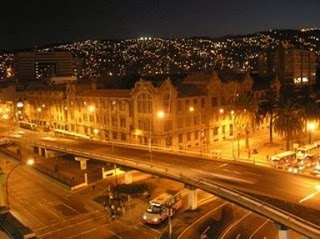
\includegraphics[width=0.6\linewidth]{Capitulo_1/imagenes/pucv.jpg} 
        \caption{Edificio PUCV.}\label{fig:pucv}
    \end{center}
\end{figure}

    \section{Capítulo 2}

\subsection{Tablas}

Los resultados se muestran en la tabla~\ref{table:resultados}...

%% https://www.tablesgenerator.com/
\begin{table}[H]
    \begin{center}
        \caption{Resultados\label{table:resultados}}
        \begin{tabular}{|l|l|l|l|l|l|l|l|}
            \hline
            Valores    & a & b & c & b & e  & f & g \\
            \hline
            Tipo 1     & 5 & 4 & 0 & 2 &  4 & 5 &  1  \\
            Tipo 2     & 1 & 3 & 0 & 3 &  8 & 9 &  9  \\
            Tipo 3     & 2 & 2 & 1 & 0 &  7 & 8 &  3  \\
            Tipo 4     & 6 & 2 & 1 & 0 &  5 & 8 &  2  \\
            \hline
        \end{tabular}
    \end{center}
\end{table}

\subsection{Ecuaciones}

La ecuación~\ref{ec:smoothing-1} muestra...

\begin{equation} \label{ec:smoothing-1}
 {f_i}_1 (S_j) = x_{0}
\end{equation} 
\begin{equation} \label{ec:smoothing-2}
 {f_i}_n (S_j) =  x_{n-1} + \beta_i {f_i}_{n-1} (S_j)
\end{equation} 

\subsection{Código}

\begin{codigojava}
public static void main(String... args) {
    System.out.println("Hola Mundo.");
}
\end{codigojava}



    % ========== Bibliografia =================
    \makereferencia{bibliography} % Nombre del archivo de refenrencia
    % \nocite{*} % Latex por defecto no muestra la referencia si no fue citada, con el comando se muestran
                 % todas las referencias

    % ========== Anexo =================
    \begin{anexos}
        \anexo{Anexo A}
    \end{anexos}


\end{document}
